\documentclass{beamer}
\usepackage{verbatim}
\usepackage{wrapfig}
\usepackage{color}
%\usetheme{Warsaw}
\usetheme[pageofpages=of,% String used between the current page and the
                         % total page count.
          bullet=circle,% Use circles instead of squares for bullets.
          titleline=true,% Show a line below the frame title.
          %titlepagelogo=opensuse,
          alternativetitlepage=true,% Use the fancy title page.
          ]{Torino}

\title{Automated Testing with openQA}
\author{\texorpdfstring{Alex-P. Natsios\newline\url{drakevr@2f30.org}}{Author}}
%\author{Alex-P. Natsios}
\institute{Fosscomm 2015 - Athens}
\date{7 Nov 2015}
\begin{document}
    \begin{frame}
       \titlepage
    \end{frame}

    \begin{frame}{\$ whoami}
        \begin{itemize}
            \item Alexandros-Panayiotis Natsios
            \item IRC Handle: Drakevr
            \item cs undergrad student @ teilar.gr
            \item openSUSE Advocate
        \end{itemize}
    \end{frame}

    \begin{frame}
        \center\huge What is openQA?
    \end{frame}

    \begin{frame}{openQA}
        \begin{itemize}
            \item Open Source distribution testing framework
            \item Can test applications or whole operating systems
            \item In either GUI or console mode
            \item was started in 2009
            \item Is now used by major distributions like openSUSE, SUSE,  Fedora 
        \end{itemize}
    \end{frame}

    \begin{frame}
        \center\huge openQA is an integral part of the development and lifecycle of the distribution
    \end{frame}

    \begin{frame}
        \center\huge full test cycle \\
        (pre-validation,validation, post-validation)
    \end{frame}

    \begin{frame}{pre-validation}
        \begin{itemize}
            \item Incoming changes are ``staged'' and tested on top of the last good build
            \item Monitored very regularly
            \item No submissions are checked in until all openQA tests pass
        \end{itemize}
    \end{frame}

    \begin{frame}{validation}
        \begin{itemize}
            \item In depth validation is done in parallel for every build
            \item More than 100 validation scenarios tested
            \item Improved performance and coverage compared to just testing manually
        \end{itemize}
    \end{frame}

    \begin{frame}{post-validation}
        \begin{itemize}
            \item Additional tests can be scheduled automatically after validation passes
            \item Builds automatically produce verified valid disk images for further testing
        \end{itemize}
    \end{frame}

    \begin{frame}{Features}
        \begin{itemize}
            \item Uses QEMU to fire up Virtual Machine Images
            \item It can capture images and act on their contents
            \item It uses libopenCV for fuzzy image matching
            \item Can generate keystrokes (lke a normal user)
            \item It is mostly written in Perl
            \item As are the tests
            \item Rulefiles are written in JSON
            \item Licensed under GPLv2
        \end{itemize}
    \end{frame}

    \begin{frame}{New Feature Highlights}
        \begin{itemize}
            \item Multi Arch Support (Intel, ppc64le, s390x, aarch64)
            \item Multi Machine Testing (incl. openvswitch)
            \item Add On Testing
            \item Remote Workers
            \item Real Hardware Testing
            \item Disk Image Creation
            \item Testing without Installation
            \item Dashboard \& Comments
        \end{itemize}
    \end{frame}

    \begin{frame}
        \center\huge Basic Consepts
    \end{frame}

    \begin{frame}
        \center\huge Jobs
    \end{frame}

    \begin{frame}{Jobs}
        One of the most important features of openQA is that it can be used to
        test several combinations of actions and configurations.
    \end{frame}

    \begin{frame}{Jobs}
        For every one of those combinations, the system creates a virtual
        machine, performs certain steps and returns an overall result.
    \end{frame}

    \begin{frame}{Jobs}
        Every one of those executions is called a job.
        Every job is labeled with a numeric identifier and has several
        associated settings that will drive its behavior.
    \end{frame}

    \begin{frame}{Jobs}
        \begin{block}{A job goes through several states:}
            \begin{itemize}
                \item {\bf scheduled} Initial state for recently created jobs. \\
                    (Queued for future execution.)
                \item {\bf running} Jobs in progress.
                \item {\bf cancelled} Jobs that have been cancelled by a user or cloned
                \item {\bf waiting} The job is in ‘interactive mode’ and waiting for input
                \item {\bf done} Finished Jobs
            \end{itemize}
        \end{block}
    \end{frame}

    \begin{frame}{Jobs}
        Jobs in state {\bf done} have typically gone through a whole sequence of 
        steps (called {\bf testmodules}) each one with its own result. \\
        But in addition to those partial results, a finished {\bf job} also 
        provides an overall result from the following list.
    \end{frame}

    \begin{frame}
        \begin{itemize}
            \item {\bf none} For jobs that have not reached the ``done'' state.
            \item {\bf passed} No critical check failed during the process.
            \item {\bf failed} At least one assertion considered to be critical was not satisfied at some point.
            \item {\bf incomplete} The job is no longer running but no result was provided. Either it was cancelled while running or it crashed.
        \end{itemize}
    \end{frame}

    \begin{frame}{Exceptions}
        Sometimes, the reason of a failure is not an error in the tested operating system itself.
        \begin{itemize}
            \item Can be an outdated test
            \item A problem in the execution of the job
            \item Other external reason
        \end{itemize}
    \end{frame}

    \begin{frame}{Recovery}
         It makes sense to re-run a given job from the beginning once the
         problem is fixed or the tests have been updated.

    \end{frame}

    \begin{frame}{Cloning}
         Every job can be superseded by a clone which is scheduled to run
         with exactly the same settings as the original job.
     \end{frame}

     \begin{frame}{Recovery}
         If the original job is still NOT in done state, then it is
         immediately cancelled and replaced by the clone.
     \end{frame}

     \begin{frame}{Recovery}
         The original job is still retained in the listing as is all the
         gathered information and results (for future ref and examination
         since its now considered outdated).
     \end{frame}

    \begin{frame}
        \center\huge Needles
    \end{frame}

    \begin{frame}{Needles}
        One of the main mechanisms for openQA to know the state of the virtual
        machine is checking the presence of some elements in the machine's `screen'.
    \end{frame}

    \begin{frame}{Needles}
         A needle specifies both the elements to search for and a list of tags
         used to decide which needles should be used at any moment.
    \end{frame}

    \begin{frame}{Needles}
        This is performed using fuzzy image matching between the screen and the so called needles.
    \end{frame}

    \begin{frame}{Needle example}
        A needle consists of a full screenshot in PNG format and a json file
        with the same name (e.g. foo.png and foo.json) containing the
        associated data, like which areas inside the full screenshot are
        relevant or the mentioned list of tags.
    \end{frame}

    \begin{frame}{Needle example}
        \scriptsize
        \verbatiminput{files/needle_example.json}
    \end{frame}

    \begin{frame}{Xterm Example}
        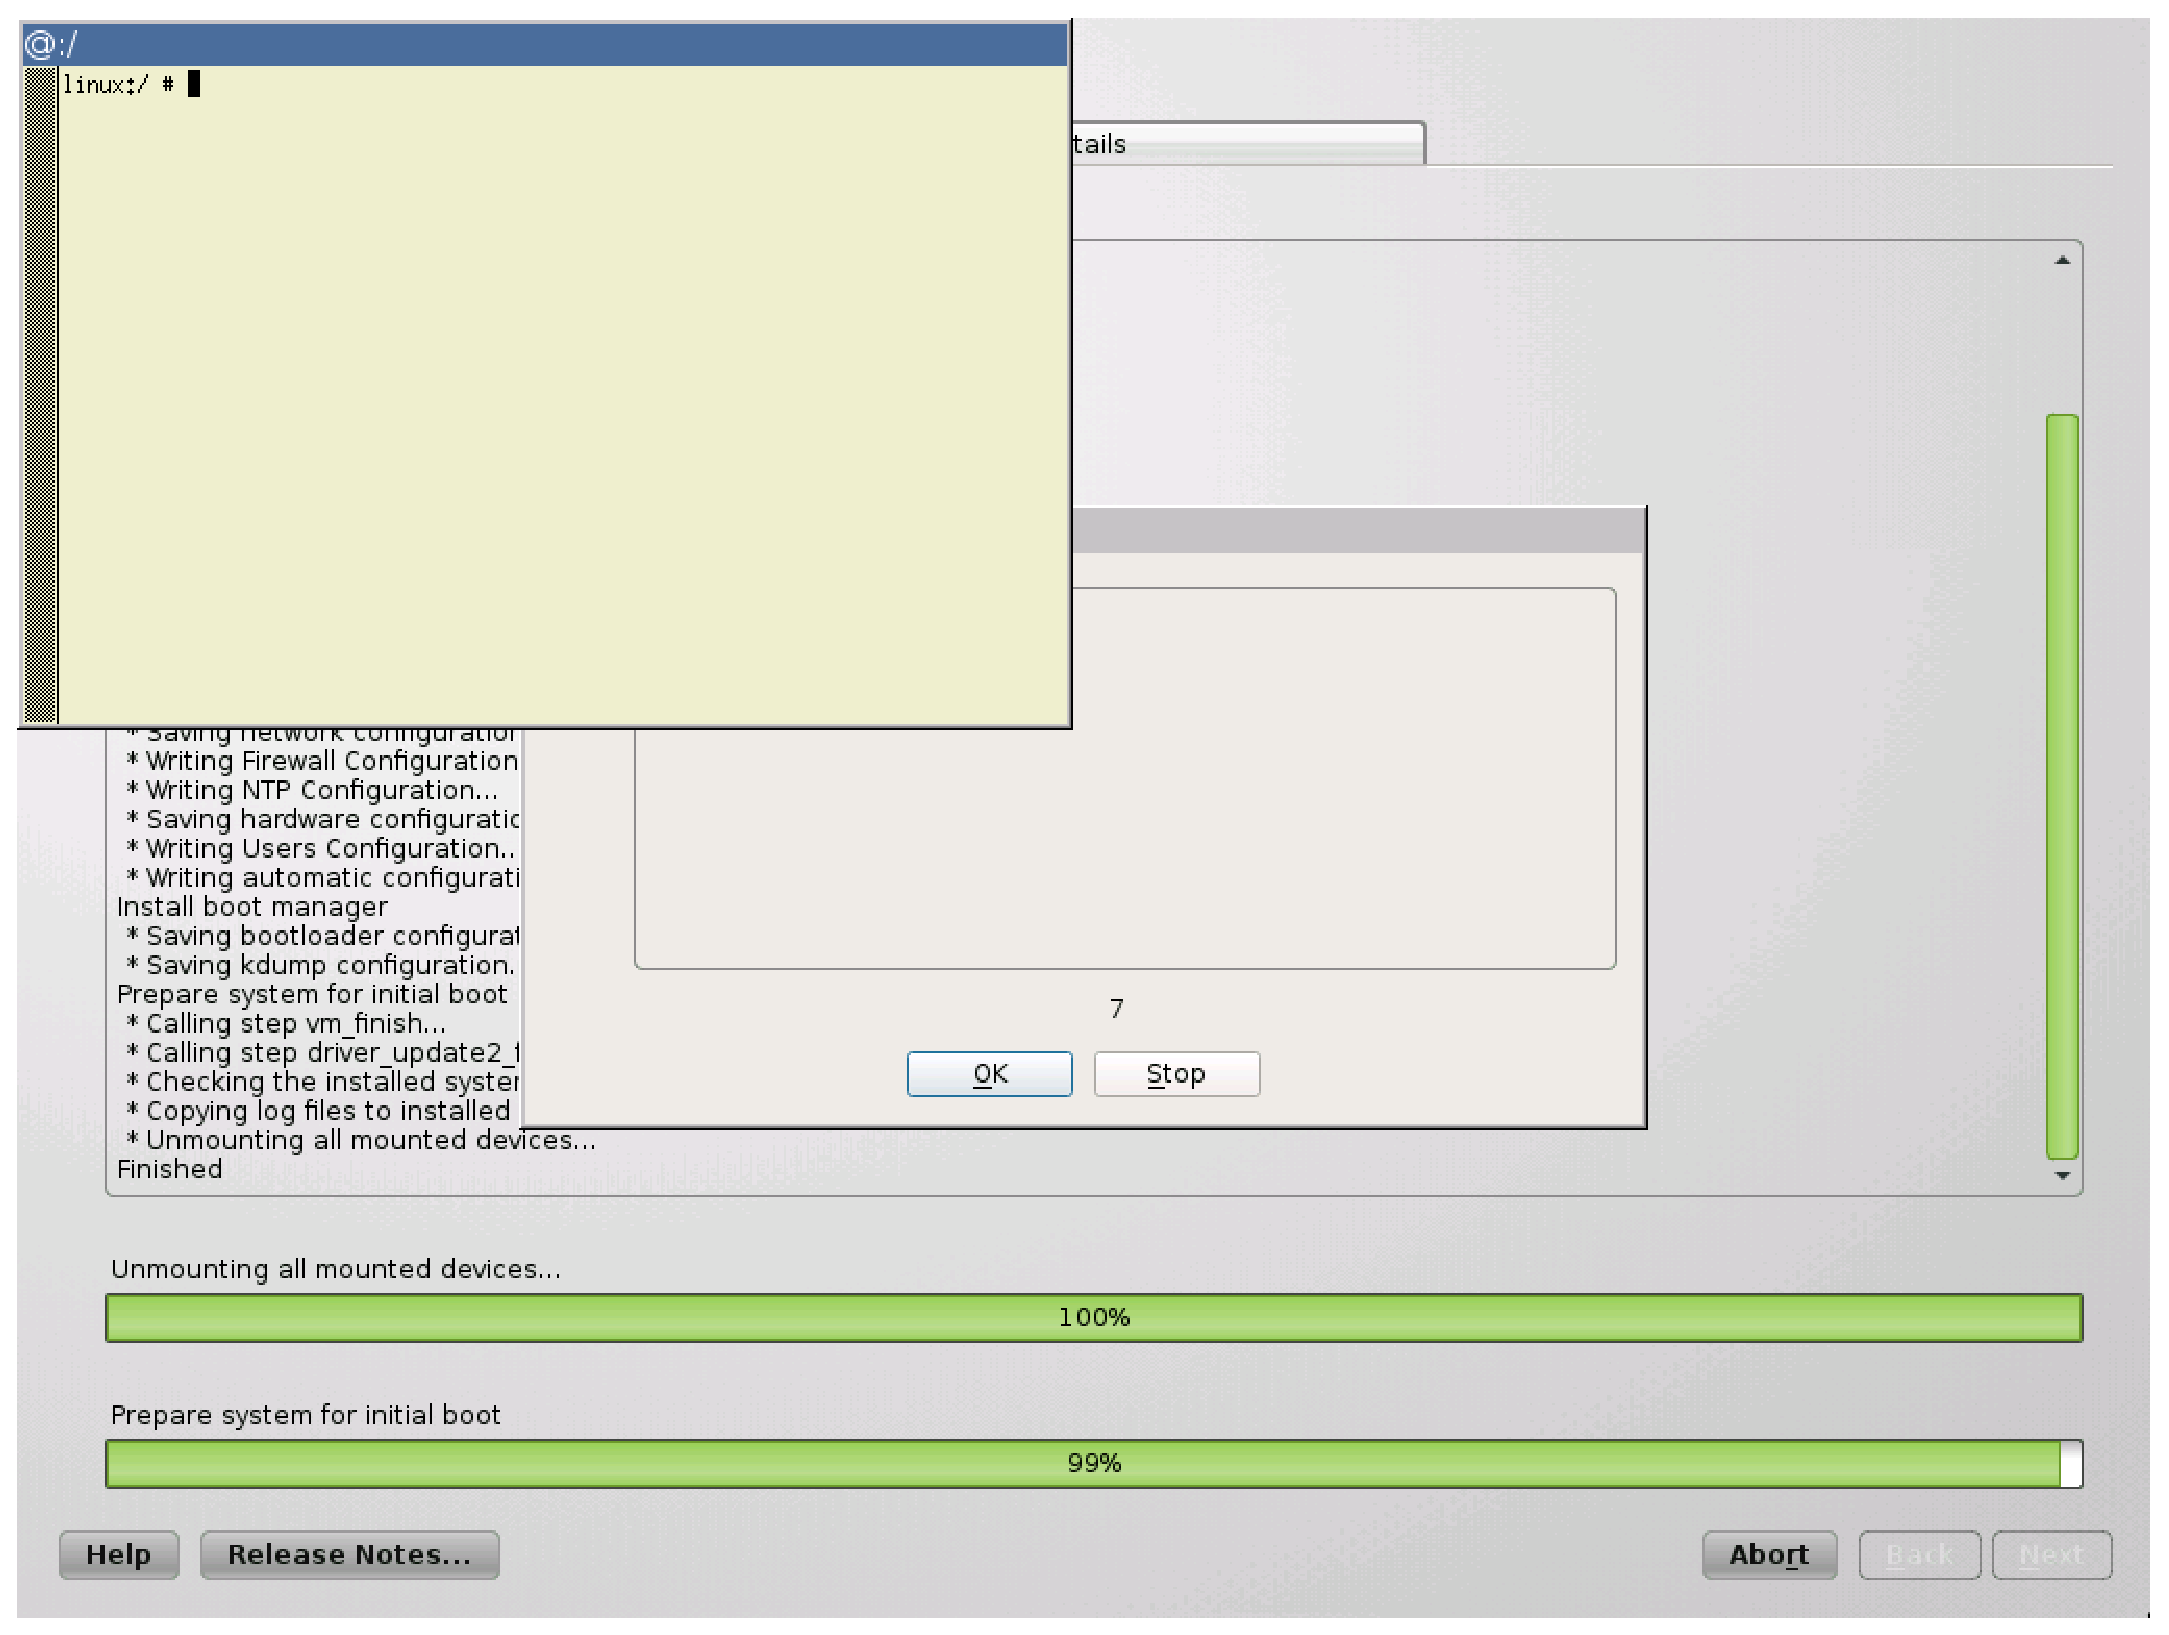
\includegraphics[scale=0.25]{files/xterm-in-yast.eps}
    \end{frame}

    \begin{frame}{Xterm Example}
        \verbatiminput{files/xterm-in-yast.json}
    \end{frame}

    \begin{frame}
        \center\huge Interactive Mode
    \end{frame}

    \begin{frame}{Interactive Mode}
        There are several points in time during the execution of a job at which
        openQA tries to match the screen with the available needles, reacting
        to the result of that check.
    \end{frame}

    \begin{frame}{Interactive Mode}
        If the job is running in interactive mode it will stop the execution at
        that point, freezing the virtual machine and waiting for user input
        before proceeding.
    \end{frame}

    \begin{frame}{Interactive Mode}
        At that moment, the user can modify the existing needles or can create
        a new one using as a starting point either the current screen of the
        virtual machine or one of the existing needles.
    \end{frame}

    \begin{frame}{Interactive Mode}
        Once the needles are adjusted, the user can command the job to reload
        the list of needles and continue with the execution.
    \end{frame}

    \begin{frame}{Interactive Mode}
        The interactive mode is especially useful when creating needles for a
        new operating system or when the look \& feel have changed and several
        needles need to be adjusted accordingly.
    \end{frame}

    \begin{frame}
        \center\huge Architecture
    \end{frame}

    \begin{frame}
        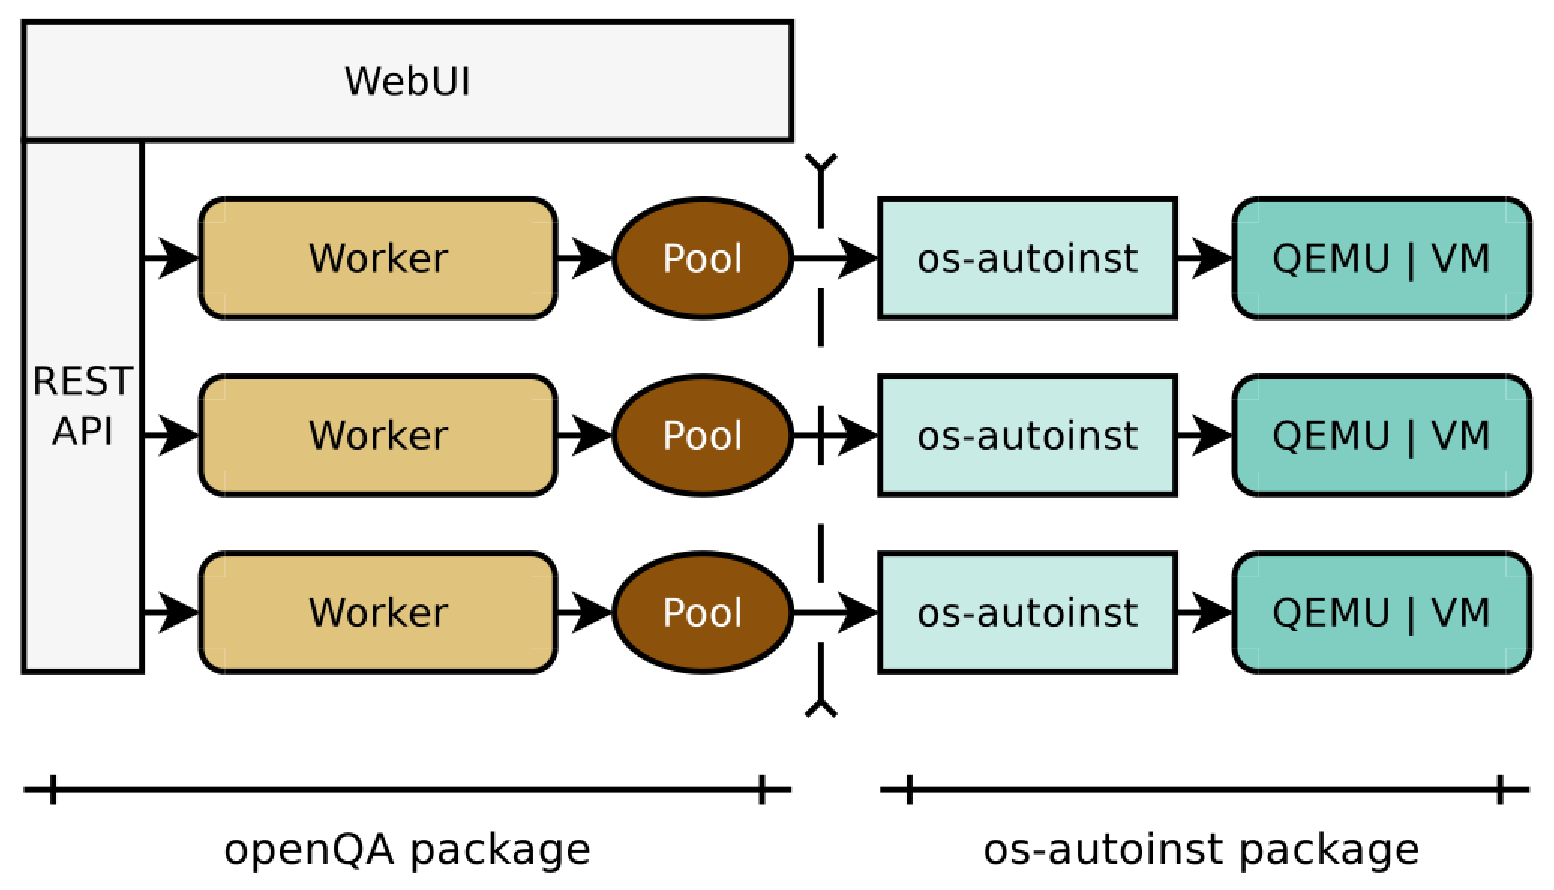
\includegraphics[scale=0.40]{files/arch.eps}
    \end{frame}

    \begin{frame}{Links}
        \begin{itemize}
            \item https://openqa.opensuse.org/ [Homepage]
            \item http://en.opensuse.org/openSUSE:OpenQA [Wiki Portal]
            \item https://github.com/os-autoinst/os-autoinst [Framework Source]
            \item https://github.com/os-autoinst/openQA [Web Interface]
        \end{itemize}
    \end{frame}

    \begin{frame}{Q \& A}{Thank you for your attention!}
        \center Alex-P. Natsios\\
        \center\url{drakevr@2f30.org}\\
        \center\url{http://drakevr.gr}\\
        \center\url{http://www.linkedin.com/in/drakevr}\\
        \center\url{http://www.github.com/drakevr}\\
        \center\url{http://www.facebook.com/drakevr}\\
        \center\url{http://www.twitter.com/drakevr}
    \end{frame}

\end{document}
